\documentclass[letterpaper]{article}

\usepackage[utf8]{inputenc}
\usepackage{fontenc}
\usepackage{graphicx}
\usepackage{caption}
\usepackage{subcaption}
\usepackage{amsmath}
\usepackage{listings}
\usepackage[top=1in,bottom=1in,left=1in,right=1in]{geometry}
\usepackage[dvips]{hyperref}

\title{Assignment 02 Report}
\author{Luke Fraser}
\date{11/24/14}

\begin{document}
\maketitle
\begin{abstract}
In this project we analyze the effects of filtering in the frequency domain. In many cases transforming data into the frequency domain allows for different types of image analysis and restoration means over the spatial domain. This can be seen especially in periodic noise removal. Performing convolution on an image is also faster in the frequency domain over the spatial domain when the two functions being convolved are roughly the same size. This report shows examples of frequency domain filtering on images to show the usefulness of the frequency domain in image processing.
\end{abstract}

\section{Noise Removal}
\begin{figure}[hbtp]
  \centering
  \begin{subfigure}{6.1cm}
    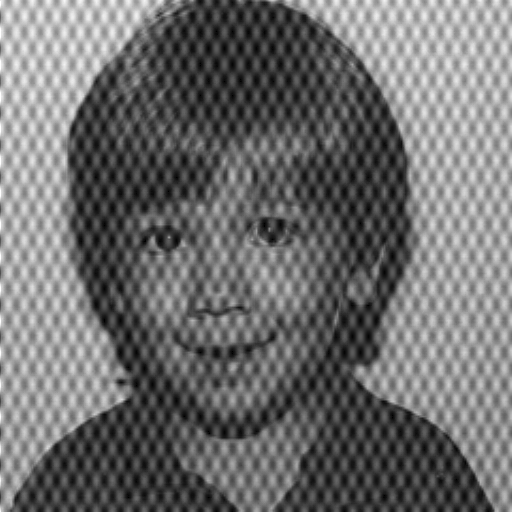
\includegraphics[width=6.1cm]{images/boy_noisy.png}
    \caption{Original Image: with cosine noise}
  \end{subfigure}
  \begin{subfigure}{6.1cm}
    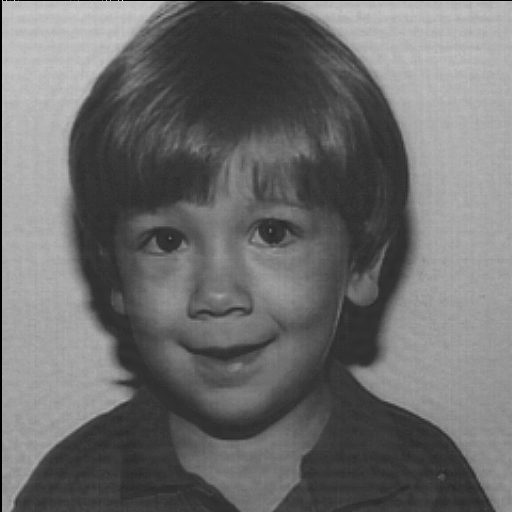
\includegraphics[width=6.1cm]{images/boy_denoise.png}
    \caption{Noise removal}
  \end{subfigure}
  \caption{Periodic noise removal	}
  \label{fig:noise_periodic}
\end{figure}
\begin{figure}[hbtp]
  \centering
  \begin{subfigure}{6.1cm}
    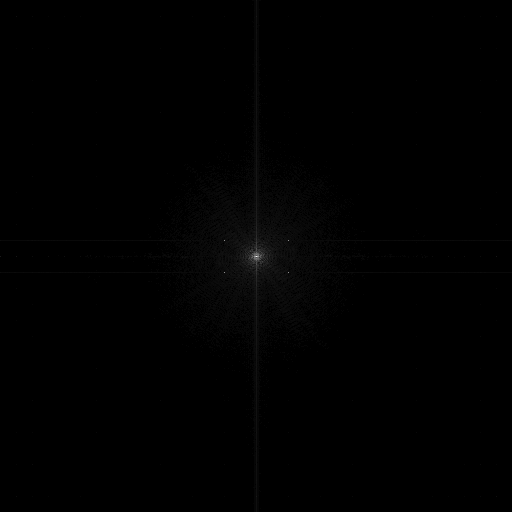
\includegraphics[width=6.1cm]{images/FT_boy_noisy.png}
    \caption{Original Imag spectrum}
  \end{subfigure}
  \caption{Boy Noise Spectrum Image}
  \label{fig:noise_periodic}
\end{figure}
Noise removal typically involves blurring and image with a low-pass filter of some kind. The typical procedure of removing noise involves convolving an image with a gaussian function with a certain variance. This produces a smoother image with high frequency information removed. If we have \emph{a priori} knowledge about the type of noise we can make smart decisions about how to remove the noise. For the case of periodic noise in an image as seen in figure~\ref{fig:noise_periodic} convolution with a Gaussian will not adequately remove the noise. In this case the frequency domain is perfect for removing repeating patterns of noise. In figure~\ref{fig:noise_periodic} an image of boy had additive noise applied the image values. The noise is cosine noise. When the image is transformed into the frequency domain the noise will appear as peaks in the spectrum of the image as seen figure~\ref{fig:noise_spectrum}. The noise can be removed cleanly with a band-reject filter in the frequency domain without effecting the rest of the image. Figure~\ref{fig:noise_periodic} is an example of applying a band-reject filter on the boy image. The noise is completely removed with much effect on the rest of the image. The filter is also able to maintain the high-frequency information of the image. This is a key distinction between filtering in the spatial domain and in the frequency domain.
\section{Convolution in the frequency domain}
\begin{figure}[hbtp]
  \centering
  \begin{subfigure}{6.1cm}
    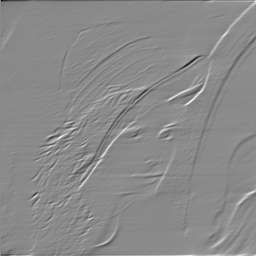
\includegraphics[width=6.1cm]{images/lenna_ft_convolve.png}
    \caption{Convolution: Frequency domain}
  \end{subfigure}
  \begin{subfigure}{6.1cm}
    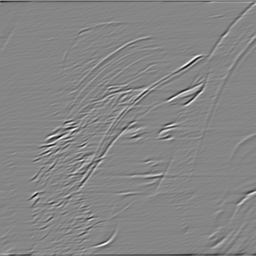
\includegraphics[width=6.1cm]{images/lenna_convolution.png}
    \caption{Convolution: Spatial domain}
  \end{subfigure}
  \caption{Convolution is both the frequency domain and the spatial domain.}
  \label{fig:convolution}
\end{figure}
An important relationship between the frequency domain and the spatial domain is the convolution theorem. Eq.~\ref{eq:convolution} shows this relationship.
\begin{equation}\label{eq:convolution}
\mathcal{F}(g*f)=\mathcal{F}(g)\mathcal{F}(f) 
\end{equation}

The relationship states that the convolution in the spatial domain is equivalent to multiplication in the frequency domain and vice versa. The convolution theorem provides a means to improve efficiency over standard convolution in the frequency domain. By performing convolution in the frequency domain major speedups can be achieved over typical sptial domain convolution espeicially when the mask size is large.

In this section a demonstration of the convolution in the frequency domain is shown. As well the difference between this operation in the spatial domain and frequency domain is shown. The Sobel mask is used to find vertical differences in the image or edges. The Sobel mask is transformed into the frequency domain and then multiplied with the FT of the image. The results as seen in figure~\ref{fig:convolution} show that multiplication in the frequency and convolution in the spatial domain are equivalent.
\section{Motion blur}
\begin{figure}[hbtp]
  \centering
  \begin{subfigure}{4cm}
    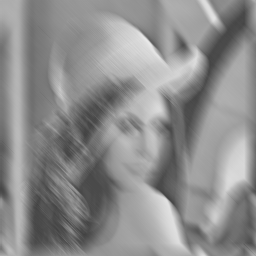
\includegraphics[width=4cm]{images/lenna_blur_0015.png}
    \caption{Motion: no noise}
  \end{subfigure}
  \begin{subfigure}{4cm}
    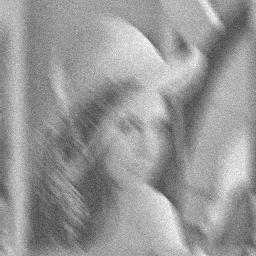
\includegraphics[width=4cm]{images/lenna_blur_10.png}
    \caption{Motion: $Noise(0,10)$}
  \end{subfigure}
  \begin{subfigure}{4cm}
    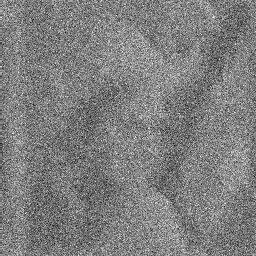
\includegraphics[width=4cm]{images/lenna_blur_100.png}
    \caption{Motion: $Noise(0,100)$}
  \end{subfigure}
  \begin{subfigure}{4cm}
    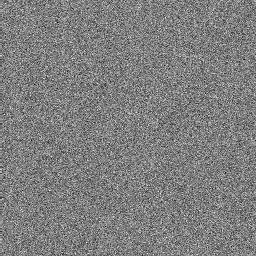
\includegraphics[width=4cm]{images/lenna_blur_1000.png}
    \caption{Motion: $Noise(0,1000)$}
  \end{subfigure}
  \caption{Motion blurred images with different additive gaussian noise applied.}
  \label{fig:motion}
\end{figure}
Artifacts in images due to motion blur are common. They can occur from a shaky camera or from different camera movements over the time of a single shutter. It is useful to model this effect in images in order to recover the original image from the blurred one. For the case of this experiment it is assumed that the motion of the image is known \emph{a priori} as well it is also assumed that the motion of the image is linear and planar. This means that the entire image exhibits the same motion blur and no effects due to parallax of a 3D scene are present. Figure~\ref{fig:motion} shows an example of such a blur. This although limiting is still very powerful model when restoring images damaged by this blur.

\begin{equation} \label{eq:motionmodel}
H(u,v)=\frac{T}{\pi (ua + ub)}sin(\pi (ua + ub))e^{-j\pi (ua + ub)}
\end{equation}
\begin{figure}[hbtp]
  \centering
  \begin{subfigure}{4cm}
    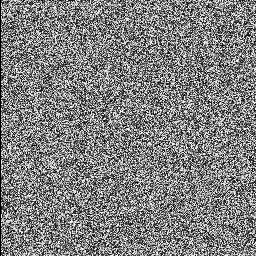
\includegraphics[width=4cm]{images/lenna_deblurred_inverse.png}
    \caption{Motion: no noise}
  \end{subfigure}
  \begin{subfigure}{4cm}
    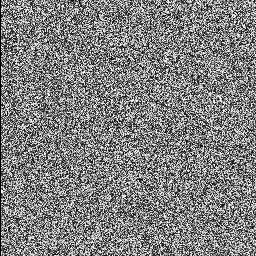
\includegraphics[width=4cm]{images/lenna_deblurred_inverse_10.png}
    \caption{Motion: $Noise(0,10)$}
  \end{subfigure}
  \begin{subfigure}{4cm}
    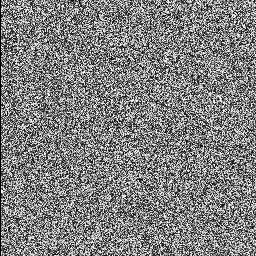
\includegraphics[width=4cm]{images/lenna_deblurred_inverse_10.png}
    \caption{Motion: $Noise(0,100)$}
  \end{subfigure}
  \begin{subfigure}{4cm}
    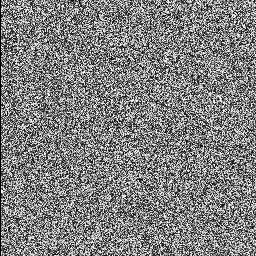
\includegraphics[width=4cm]{images/lenna_deblurred_inverse_10.png}
    \caption{Motion: $Noise(0,1000)$}
  \end{subfigure}
  \caption{Motion blurred images with different additive gaussian noise applied.}
  \label{fig:inverse}
\end{figure}
In this section two methods of removing motion blur from an image are tested: inverse filtering and Weiner filtering. Inverse filtering is the naive approach to removing noise based on the motion model described in eq.~\ref{eq:motionmodel} and can seen in eq~\ref{eq:inverse}.
\begin{equation} \label{eq:inverse}
\hat{F}(u,v)=\frac{G(u,v)}{H(u,v)}
\end{equation}
\begin{figure}[hbtp]
  \centering
  \begin{subfigure}{4cm}
    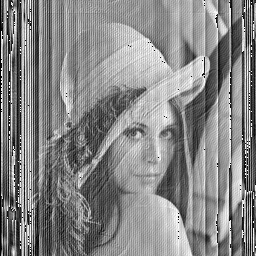
\includegraphics[width=4cm]{images/lenna_deblur_0015.png}
    \caption{Weiner: no noise}
  \end{subfigure}
  \begin{subfigure}{4cm}
    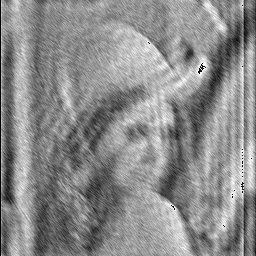
\includegraphics[width=4cm]{images/lenna_deblurred_weiner_10.png}
    \caption{Weiner: $Noise(0,10)$}
  \end{subfigure}
  \begin{subfigure}{4cm}
    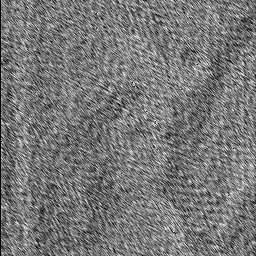
\includegraphics[width=4cm]{images/lenna_deblurred_weiner_100.png}
    \caption{Weiner: $Noise(0,100)$}
  \end{subfigure}
  \begin{subfigure}{4cm}
    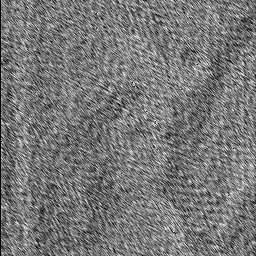
\includegraphics[width=4cm]{images/lenna_deblurred_weiner_100.png}
    \caption{Weiner: $Noise(0,1000)$}
  \end{subfigure}
  \caption{Weiner filter applied to images of different motion blur and noise.}
  \label{fig:weiner}
\end{figure}
The main dsadvantage to inverse filtering is that it doesn't take into account the noise of an image. Inverse filtering is very sensitive to noise and other methods must be used to acheive better results. Weiner filtering was devised for this specific reason and eq~\ref{eq:weiner} shows the method. 
\begin{equation} \label{eq:weiner}
\hat{F}(u,v)=\frac{|H(u,v)|^2}{|H(u,v)|^2 +k} * \frac{G(u,v)}{H(u,v)}
\end{equation}

The $K$ parameter is used to estimate the effects of noise on the image. This parameter must be tuned to find a value that best suits the blur of the image. figure~\ref{fig:inverse} shows the results of inverse filtering on the lenna image with different levels of noise added to the image. Unfortunately I was unable to achieve working results with the inverse filter. As well figure~\ref{fig:weiner} shows the results of Weiner filtering at different levels of noise. It can be seen how much the Weiner method out performs the inverse filtering method. It is very important to consider noise in when dealing with real world images. It is unlikely that inverse would work in any real world situation.
\section{Homomorphic filtering}
\begin{figure}[hbtp]
  \centering
  \begin{subfigure}{4cm}
    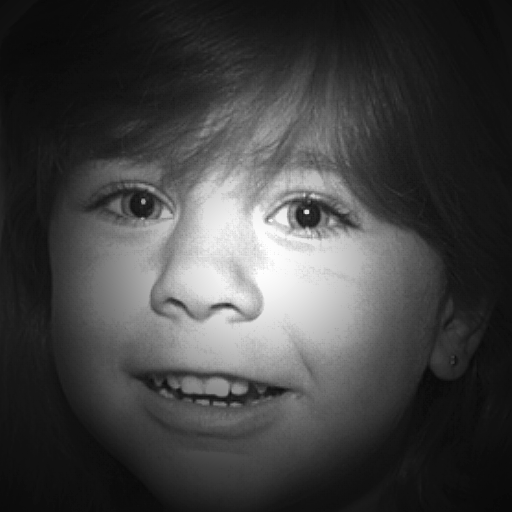
\includegraphics[width=4cm]{images/girl.png}
    \caption{Weiner: no noise}
  \end{subfigure}
  \begin{subfigure}{4cm}
    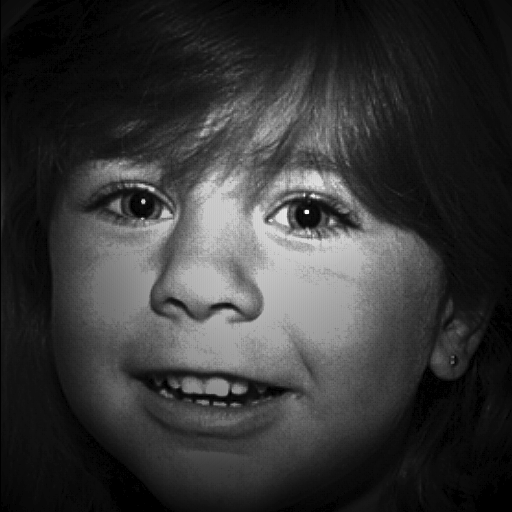
\includegraphics[width=4cm]{images/girl_homo_0_8_1_2_1_8.png}
    \caption{Weiner: $Noise(0,10)$}
  \end{subfigure}
  \begin{subfigure}{4cm}
    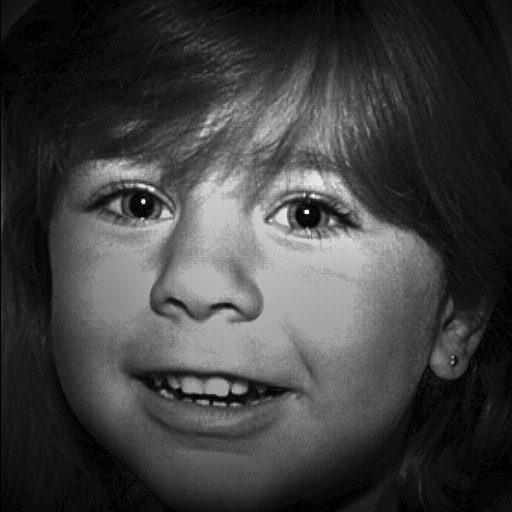
\includegraphics[width=4cm]{images/girl_homo_0_5_1_2_1_8.png}
    \caption{Weiner: $Noise(0,100)$}
  \end{subfigure}
  \begin{subfigure}{4cm}
    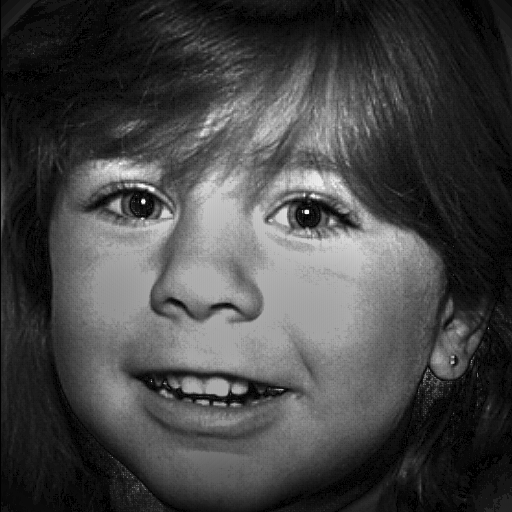
\includegraphics[width=4cm]{images/girl_homo_best.png}
    \caption{Weiner: $Noise(0,1000)$}
  \end{subfigure}
  \caption{Weiner filter applied to images of different motion blur and noise.}
  \label{fig:weiner}
\end{figure}
Homomorphic filtering is a very useful method for restoring images with uneven illumination. It takes advantage of an radiance model represented by eq~\ref{eq:illum}.
\begin{equation} \label{eq:illum}
f(x,y)=I(x,y)R(x,y)
\end{equation}
This is a simple, but powerful model that is true in many cases. $I(x,y)$ is the illumination component and $R(x,y)$ is the reflectance component and the two multiply to produce the final image. This assumption allows the contributions of the each component to be separated out in the image using the $log(I*R)$. By doing this and then performing a highpass filter a smoothing of the illumination in the image can be obtained. Eq~\ref{eq:homo} shows how a filter can be applied that will affect each component separately. The basic algorithm is listed below.
\begin{equation} \label{eq:homo}
ln(f(x,y))h(x,y)=ln(I(x,y))h(x,y) +ln(R(x,y))h(x,y)
\end{equation}


The results of the homomorphic are shown in figure~\ref{fig:homo} with different high-pass filters applied. A ButterWorth filter was used to perform the high-pass filter int he frequency domain. Different results are achieved with different values of the butterworth filter. Eq~\ref{eq:butter} represents the butterworth filter generator used.
\begin{align} \label{eq:butter}
&H(u,v)=\gamma_{L}+\frac{\gamma_{H}}{1 + [\frac{D_{0}}{D}]^2} \\
& D = \sqrt{(u-N/2)^2+(v-N/2)^2} \nonumber
\end{align}

  
\end{document}